%%%%%%%%%%%%%%%%%%%%%%%%%
\section{\label{sec:rhs_npt}Unbiased isothermal-isobaric ensemble trials}
%%%%%%%%%%%%%%%%%%%%%%%%%

Isothermal-isobaric ensemble trials change the volume, $V$, with constant number of particles, $N$, pressure, $P$ and temperature, $T$.
Volume-change trials are conducted while simultaneously scaling the coordinates of the particles uniformly.
This is done for a variety of reasons that are discussed in Section~\ref{sec:lhs_dv}.
In order to derive the appropriate MC acceptance criteria for this trial, the microstate probability must be expressed in scaled coordinates given by $s_d = r_d/L_d$, where $d$ is the dimensionality of the system.
In the following two sections, we consider the $NPT$ ensemble both without and with a ``shell" particle~\cite{koper_length_1996, corti_deriving_1998, hatch_theory_2024}, where a shell particle is used to remove redundant microstates from the isothermal-isobaric ensemble partition function.

%%%%%%%%%%%%%%%%%%%%%%%%%
\subsection{\label{sec:rhs_npt_shell}Isothermal-isobaric ($NPT$) ensemble without a shell particle}
%%%%%%%%%%%%%%%%%%%%%%%%%

The microstate probability in the $NPT$ ensemble without a shell particle is proportional to \cite{wood_monte_1968, allen_computer_1989, frenkel_understanding_2002}
\begin{equation}
\Pi \diff\mathbf{s}^{N}\diff\boldsymbol{\omega}^{N}\diff V \propto V^{N} e^{-\beta(U+P V)} \diff\mathbf{s}^{N} \diff\boldsymbol{\omega}^{N}\diff V.
\label{eq:rhs_npt_pi}
\end{equation}
The ratio of microstate probabilities, the first ratio in Eq.~\ref{eq:detailed_balance}, is given by
\begin{equation}
\frac{\Pi_n}{\Pi_o} = \left(\frac{V_n}{V_o}\right)^{N}e^{-\beta(\Delta U + P\Delta V)},
\label{eq:rhs_npt_delta_v}
\end{equation}
for trials that select random changes uniformly in $V$, because $V$ is the explicit variable in Eq.~\ref{eq:rhs_npt_pi}.
If an $NVT$ trial is attempted in the $NPT$ ensemble, $\Delta V=0$, and Eq.~\ref{eq:rhs_npt_pi} reduces to Eq.~\ref{eq:rhs_nvt}.

Eq.~\ref{eq:rhs_npt_pi} and \ref{eq:rhs_npt_delta_v} no longer apply if changes are uniform in $\ln V$ instead of $V$.
In this case, substituting $\diff V=V\diff\ln V$ into Eq.~\ref{eq:rhs_npt_pi}, the first ratio in Eq.~\ref{eq:detailed_balance} is
\begin{equation}
\frac{\Pi_n}{\Pi_o} = \left(\frac{V_n}{V_o}\right)^{N+1}e^{-\beta(\Delta U + P\Delta V)}.
\label{eq:rhs_npt_delta_lnv}
\end{equation}
See Code Block~\ref{sim:ideal_gas_npt} for a test of Eqs.~\ref{eq:rhs_npt_delta_v} and \ref{eq:rhs_npt_delta_lnv}.

%%%%%%%%%%%%%%%%%%%%%%%%%
\subsection{\label{sec:lhs_dv}Isotropic volume change trial}
%%%%%%%%%%%%%%%%%%%%%%%%%

Trial moves that attempt isotropic volume changes proceed as follows.
The positions of the particles and periodic boundary lengths are scaled by a factor of $(1+\Delta V/V_o)^{1/D}$ in each of $D$ dimensions, where $\Delta V$ is chosen as a random amount selected uniformly within $\pm\Delta V_{\mathrm{max}}$.
The particle positions are typically scaled with the volume in off lattice simulations.
Careful consideration of exactly how volume is changed is required.
For example, as shown in Fig.~\ref{fig:npt}, if particle positions are wrapped during volume changes that do not scale the positions, then detailed balance may be violated.
This trial is summarized in Table~\ref{tab:lhs_dv}.

\begin{figure}
\begin{centering}
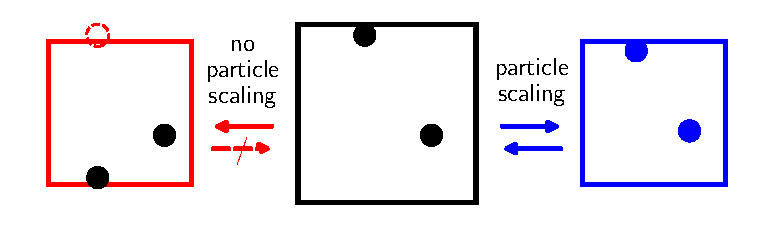
\includegraphics[width=8.5cm]{../figures/npt.pdf}
\caption{
Detailed balance is violated if the particle positions are not scaled with the volume and one of the particles is wrapped across periodic boundaries.
On the left, the top-most particle is wrapped to the bottom due to the decrease in volume when particle positions are not scaled.
The reverse move, a subsequent increase in volume without scaling, will not return the system to its original microstate, shown in the center.
On the right, detailed balance is obeyed when the particle positions are scaled with the volume.
}
\label{fig:npt}
\end{centering}
\end{figure}

\begin{table}
\begin{center}
\begin{tabular}{|c|c|}
 \hline
 \thead{Forward} & \thead{$\alpha_{o\rightarrow n}$} \\ [0.5ex]
 \hline
 \makecell{Choose $\Delta V$} & \makecell{$\diff\mathbf{r}/(2\Delta V_{\mathrm{max}})$} \\
 \hline\hline
 \thead{Reverse} & \thead{$\alpha_{n\rightarrow o}$}\\ [0.5ex]
 \hline
 \makecell{Choose $-\Delta V$} & \makecell{$\diff\mathbf{r}/(2\Delta V_{\mathrm{max}})$} \\
 \hline
\end{tabular}
\caption{Volume change transition probabilities.}
\label{tab:lhs_dv}
\end{center}
\end{table}

Substituting Eq.~\ref{eq:rhs_npt_delta_v} (without a shell particle) into Eq.~\ref{eq:detailed_balance}, and using Table~\ref{tab:lhs_dv} for the second ratio in Eq.~\ref{eq:detailed_balance} results in
\begin{equation}
\chi=\left(\frac{V_n}{V_o}\right)^{N}e^{-\beta(\Delta U + P\Delta V)}.
\label{eq:lhs_dv}
\end{equation}
This equation is also valid for uniform changes in one of the side lengths, $L_d$, with scaled particle positions because $dV \propto \diff L_d$ in Eq.~\ref{eq:rhs_npt_pi} results in the same Eq.~\ref{eq:rhs_npt_delta_v} for the first ratio in Eq.~\ref{eq:detailed_balance}.

Eq.~\ref{eq:lhs_dv} is not valid for uniformly random changes in $\ln V$.
Specifically, uniform changes in $\ln V$ occur when the particle coordinates and periodic boundary lengths are scaled by a factor of $e^{(\delta\ln V)/D}$, where $\delta\ln V$ is chosen as a random amount selected uniformly within $\pm\delta\ln V_{\mathrm{max}}$, and $\Delta V = V_o(e^{\delta\ln V}-1)$.
As discussed in Ref.~\cite{frenkel_understanding_2002} (without a shell particle) and Ref.~\cite{corti_monte_2002} and Section~\ref{sec:rhs_npt} (with a shell particle), uniform changes in $\ln V$ use Eq.~\ref{eq:rhs_npt_delta_lnv} instead of Eq.~\ref{eq:rhs_npt_delta_v}, resulting in the following acceptance probability
\begin{equation}
\chi=\left(\frac{V_n}{V_o}\right)^{N+1}e^{-\beta(\Delta U + P\Delta V)}.
\label{eq:lhs_dlnv}
\end{equation}
Code Block~\ref{sim:ideal_gas_npt} uses Eq.~\ref{eq:lhs_dv} or Eq.~\ref{eq:lhs_dlnv} for an ideal gas to compare against theory for uniform changes in $V$ or $\ln V$, respectively.

\begin{figure}
\lstinputlisting[
language=Python,
label={sim:ideal_gas_npt},
caption={MC simulation of an ideal gas in the $NPT$ ensemble using Python 3 with a shell particle and uniform changes in $V$ or $\ln V$, and the statistics module is provided in Section~\ref{sec:block_av}.}
]{../codes/ideal_gas_npt.py}
\end{figure}

%%%%%%%%%%%%%%%%%%%%%%%%%
\subsection{\label{sec:rhs_npt_no_shell}Isothermal-isobaric ensemble with a shell particle}
%%%%%%%%%%%%%%%%%%%%%%%%%

If a shell particle is introduced to remove redundant microstates in the partition function~\cite{attard_density_1995, koper_length_1996, corti_deriving_1998, han_isothermal-isobaric_2001, corti_isothermal-isobaric_2001, corti_monte_2002, stroker_systematic_2021, hatch_theory_2024}, then there is one less particle that is scaled by the volume and Eqs.~\ref{eq:rhs_npt_pi}, \ref{eq:rhs_npt_delta_v} and \ref{eq:rhs_npt_delta_lnv} become
\begin{equation}
\Pi \diff\mathbf{s}^{N-1}\diff\boldsymbol{\omega}^{N}\diff V \propto V^{N-1} e^{-\beta(U+P V)} \diff\mathbf{s}^{N-1} \diff\boldsymbol{\omega}^{N}\diff V,
\end{equation}
\begin{equation}
\frac{\Pi_n}{\Pi_o} = \left(\frac{V_n}{V_o}\right)^{N-1}e^{-\beta(\Delta U + P\Delta V)},
\end{equation}
and
\begin{equation}
\frac{\Pi_n}{\Pi_o} = \left(\frac{V_n}{V_o}\right)^{N}e^{-\beta(\Delta U + P\Delta V)},
\end{equation}
respectively.
The acceptance probabilities shown in Section \ref{sec:lhs_dv} without a shell particle would change according to these new microstate probabilities when a shell particle is included.
Specifically, Eqs.~\ref{eq:lhs_dv} and \ref{eq:lhs_dlnv} become
\begin{equation}
\chi=\left(\frac{V_n}{V_o}\right)^{N-1}e^{-\beta(\Delta U + P\Delta V)}.
\end{equation}
and
\begin{equation}
\chi=\left(\frac{V_n}{V_o}\right)^{N}e^{-\beta(\Delta U + P\Delta V)},
\end{equation}
for uniform changes in $V$ and $\ln V$, respectively.
